% The solution to the last exercise of session 1: deriving Equation 6 of the
% session 1 notebook from Equations 1 and 2. Build with: latexmk -pdf
\documentclass[11pt,a4paper]{article}

\usepackage[T1]{fontenc}
\usepackage[sfdefault]{inter}   % the slides' text face; maths keeps the KaTeX-like serif
\usepackage{mathtools}
\usepackage[margin=2.2cm]{geometry}
\usepackage{microtype}
\usepackage{xcolor}
\usepackage[most]{tcolorbox}
\usepackage{pgfplots}
\usepgfplotslibrary{groupplots}
\pgfplotsset{compat=1.18}

% the course palette, docs/assets/theme.css
\definecolor{ink}{HTML}{14171A}
\definecolor{muted}{HTML}{5B6670}
\definecolor{rule}{HTML}{E2E6EA}
\definecolor{neutral}{HTML}{7D868D}
\definecolor{accent}{HTML}{0E7C86}

\color{ink}
\setlength{\parindent}{0pt}
\setlength{\parskip}{0.6em}

% the slides' takeaway: a teal bar on the left, no fill
\newtcolorbox{takeaway}{enhanced, frame hidden, interior hidden, boxrule=0pt,
  borderline west={3pt}{0pt}{accent}, left=12pt, right=0pt, top=2pt, bottom=2pt,
  before skip=1em, after skip=1em}

\begin{document}

{\LARGE\bfseries Understanding learning rates as weighted sums\par}
\vspace{0.3em}
{\large\color{muted} Session 1: deriving Equation 6, step by step\par}
\vspace{1em}

\section*{Where we start}

In session 1 the model learns the probability that green will be rewarded with two equations.
On each trial it calculates a prediction error,
\begin{equation*}
  \underbrace{\delta_t}_\textrm{prediction error} = \underbrace{o_t}_\textrm{outcome}
  - \underbrace{p_t}_\textrm{model prediction} \tag{Equation 1}
\end{equation*}
and uses it to update its expectation:
\begin{equation*}
  \underbrace{p_{t+1}}_\textrm{new prediction} = \underbrace{p_t}_\textrm{old prediction}
  + \underbrace{\alpha \delta_t}_\textrm{scaled prediction error} \tag{Equation 2}
\end{equation*}
Here $o_t$ is the outcome on trial $t$ (1 if green was rewarded, 0 if orange was rewarded),
$p_t$ is the current estimate of the probability that green will be rewarded, and $\alpha$ is the
learning rate, with $0 < \alpha \leq 1$.

These equations only ever look one trial back. Yet the notebook claims that the prediction
depends on \emph{every} past outcome, as a weighted sum:
\begin{equation*}
  p_{T+1} = (1-\alpha)^T p_1 + \sum^T_{t=1} w_t o_t \tag{Equation 5}
\end{equation*}
with weights
\begin{equation*}
  w_t = \alpha(1-\alpha)^{T-t} \tag{Equation 6}
\end{equation*}
where $T$ is the current trial and $T-t$ is how many trials into the past we are looking.
This handout shows where these two equations come from.

\section*{Step 1: Combine Equations 1 and 2 into one}

Put the prediction error from Equation 1 into Equation 2, and collect the two terms that
contain $p_t$:
\begin{align*}
  p_{t+1} &= p_t + \alpha(o_t - p_t) \\
          &= p_t - \alpha p_t + \alpha o_t \\
          &= (1-\alpha)\, p_t + \alpha o_t .
\end{align*}
This already says something useful: the new prediction is a \emph{mix} of the old prediction
and the newest outcome. With $\alpha = 0.3$, for example, it is 70\% old prediction and 30\% new
outcome.

\section*{Step 2: Apply the rule trial by trial}

The model starts with a prediction $p_1$ on the first trial (\texttt{startingProb}, 0.5 by
default). Now apply the rule from Step 1 over and over. Each time, replace the previous
prediction with what the line above already worked out for it.

\textbf{After one trial:}
\begin{equation*}
  p_2 = (1-\alpha)\, p_1 + \alpha o_1 .
\end{equation*}

\textbf{After two trials:}
\begin{align*}
  p_3 &= (1-\alpha)\, p_2 + \alpha o_2 \\
      &= (1-\alpha) \underbrace{\bigl[(1-\alpha)\, p_1 + \alpha o_1\bigr]}_{p_2} + \alpha o_2 \\
      &= (1-\alpha)^2 p_1 + \alpha(1-\alpha)\, o_1 + \alpha o_2 .
\end{align*}

\textbf{After three trials:}
\begin{align*}
  p_4 &= (1-\alpha)\, p_3 + \alpha o_3 \\
      &= (1-\alpha) \underbrace{\bigl[(1-\alpha)^2 p_1 + \alpha(1-\alpha)\, o_1
         + \alpha o_2\bigr]}_{p_3} + \alpha o_3 \\
      &= (1-\alpha)^3 p_1 + \alpha(1-\alpha)^2 o_1 + \alpha(1-\alpha)\, o_2 + \alpha o_3 .
\end{align*}

A pattern is appearing. Read the last line from right to left:
\begin{itemize}
  \item the outcome of the \emph{last} trial, $o_3$, is multiplied by $\alpha$;
  \item the outcome one trial before that, $o_2$, by $\alpha(1-\alpha)$;
  \item the outcome two trials before that, $o_1$, by $\alpha(1-\alpha)^2$;
  \item and the starting prediction $p_1$ by $(1-\alpha)^3$.
\end{itemize}
Each step back in time adds one more factor of $(1-\alpha)$.

\section*{Step 3: The pattern holds on every trial}

The pattern carries on for any number of trials, and the reason is simple. Every new trial does
the same two things: it multiplies \emph{everything already in the prediction} by $(1-\alpha)$,
and it adds the newest outcome multiplied by $\alpha$. So an outcome from one trial further back
has picked up exactly one more factor of $(1-\alpha)$.

After $T$ trials, the outcome of trial $t$ lies $T-t$ trials in the past, so it has picked up
$T-t$ factors of $(1-\alpha)$, and the starting prediction has picked up $T$ of them. That is
Equations 5 and 6:
\begin{takeaway}
\centering
$\displaystyle
  p_{T+1} = \underbrace{(1-\alpha)^T p_1}_{\substack{\textrm{what is left of the}\\
                                                    \textrm{starting prediction}}}
  + \sum^T_{t=1} \underbrace{\alpha(1-\alpha)^{T-t}}_{w_t}\, o_t$
\end{takeaway}

The symbol $\sum$ means ``add up''. Here it says: for every trial $t$ from 1 to $T$, multiply
its outcome by its weight $w_t$, and add the results together. Written out for $T = 3$, it is
exactly what we found for $p_4$:
\begin{equation*}
  \sum^3_{t=1} \alpha(1-\alpha)^{3-t} o_t
  = \alpha(1-\alpha)^2 o_1 + \alpha(1-\alpha)\, o_2 + \alpha o_3 .
\end{equation*}

\section*{What this tells us}

\paragraph{Older outcomes count less.}
Because $1-\alpha$ is less than 1, each step back multiplies the weight by the same factor
$1-\alpha$, so the weights shrink steadily. The last trial carries weight $\alpha$.

\begin{center}
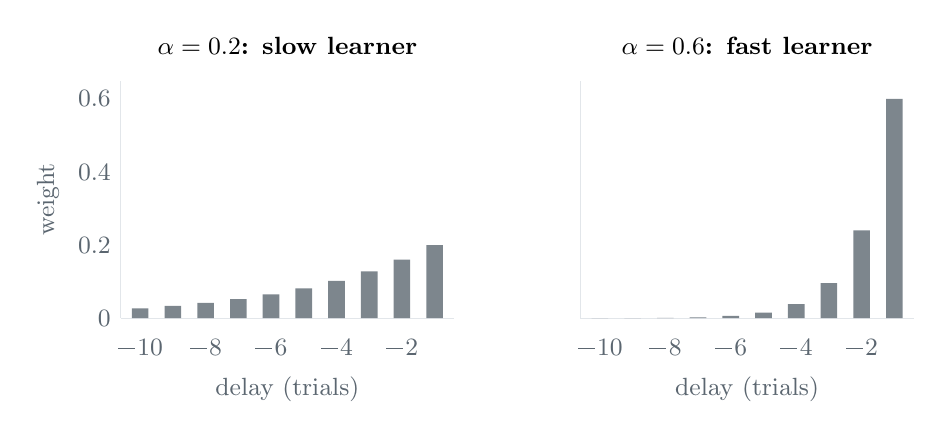
\begin{tikzpicture}
  \begin{groupplot}[
      group style={group size=2 by 1, horizontal sep=1.6cm, y descriptions at=edge left},
      width=0.48\linewidth, height=4.6cm,
      ybar, /pgf/bar width=6pt,
      ymin=0, ymax=0.65, xmin=-10.6, xmax=-0.4,
      xtick={-10,-8,...,-2}, xticklabels={\textminus10,\textminus8,\textminus6,\textminus4,\textminus2}, ytick={0,0.2,0.4,0.6},
      xlabel={delay (trials)}, ylabel={weight},
      axis lines*=left, axis line style={rule},
      tick style={draw=none}, tick label style={font=\small, color=muted},
      /pgf/number format/assume math mode=true,
      label style={font=\small, color=muted},
      title style={font=\small\bfseries},
    ]
    \nextgroupplot[title={$\alpha = 0.2$: slow learner}]
      \addplot[fill=neutral, draw=none, samples at={-10,...,-1}] {0.2*(0.8)^(-x-1)};
    \nextgroupplot[title={$\alpha = 0.6$: fast learner}]
      \addplot[fill=neutral, draw=none, samples at={-10,...,-1}] {0.6*(0.4)^(-x-1)};
  \end{groupplot}
\end{tikzpicture}
\end{center}

A fast learner (large $\alpha$) bases its prediction almost entirely on the last few outcomes.
It adapts quickly when the reward probability changes, but every chance outcome throws it around.
A slow learner (small $\alpha$) spreads its weight over a long stretch of the past. Its
prediction is steadier, but it takes longer to catch up after a change. With $\alpha = 1$, only
the last outcome counts.

\paragraph{The starting prediction is forgotten.}
$p_1$ is multiplied by $(1-\alpha)^T$, which shrinks towards zero as trials go by. With
$\alpha = 0.2$, after 20 trials only $0.8^{20} \approx 0.01$ of it is left, so the starting
probability hardly matters once there are enough trials.

\paragraph{The weights add up to 1.}
Suppose the starting prediction is $p_1 = 1$ and green is rewarded on every trial. Then every
prediction error is $1 - 1 = 0$, so the prediction never moves and stays at 1. In Equation 5,
every $o_t$ and $p_1$ is then 1, so the right-hand side is just the sum of all the weights.
Since the left-hand side is 1,
\begin{equation*}
  (1-\alpha)^T + \sum^T_{t=1} w_t = 1 .
\end{equation*}
The prediction is therefore a weighted \emph{average} of zeros and ones, which is why it always
stays between 0 and 1, as a probability must.

\end{document}
